%%==================================================
%% chapter2.tex for BIT Master Thesis
%% version: 0.1
%% last update: Nov 8th, 2017
%%==================================================
\chapter{半参数系统与信息浓缩估计}\label{chap:2}

传统鲁棒控制主要考虑小范围的结构不确定性,传统自适应控制主要考虑系统的参数不确定性,而一般的非线性自适应控制直接考虑非线性模型从而设计复杂的控制器。实际问题中参数不确定性和较大的结构不确定性可同时出现,因此这些方法对于解决非线性不确定性被控对象的离散时间控制问题都存在一定的局限性。所有的被控对象本质上都是非线性的,但是线性控制方法在反馈控制前期发展中起到了很大作用。这不由得让人思考,是否很多非线性对象都存在一个起主要作用的线性模型?按照这个思路,虽然无法精确的已知非线性不确定性系统的离散化模型,但是这些非线性系统可以用一个线性模型(如ARX模型)加上一个非线性部分(关于输入输出数据的未知函数)近似,也就是把系统的不确定性分为参数和非参数不确定性。为了解决控制问题,需要先辨识参数部分。这就是本章要介绍的半参数系统和所谓的信息浓缩(information concentration estimate, IC)估计。

\section{反馈机制能力极限的探索}\label{sect:2.1}
不管是采用连续时间模型还是离散时间角度设计控制律,实际系统都会存在无法预测的不确定性,如干扰、未建模动态等,这会导致输出就会产生偏差。反馈从一开始就是为了解决这种偏差和不确定性而引入的。传统针对线性时不变系统设计的控制方法属于线性反馈。然而,即便是针对ARX模型设计的自校正调节器,自适应控制从本质上说是一种非线性反馈\upcite{Guo2003}。当系统存在不确定性时,在设计自适应辨识与控制算法时,是否一定存在一种自适应控制律能够使得系统闭环稳定?这是在设计自适应控制之前首先要回答的问题。然而直到20世纪90年代末,郭雷院士等学者开始探索反馈机制\upcite{Guo1997},创造性地提出反馈机制的最大能力和局限(the limit to the capability of feedback)这一重要命题,并针对一些基本控制系统的自适应反馈极限进行定量研究,才引起来广泛的关注。

最开始关于反馈机制的研究始于一类基本的不确定非线性系统,即下面的模型
\begin{equation}%
\label{eq:Guo1}
y_{k+1} = \theta \phi_{k} + u_{k} + \omega_{k+1},\ \phi_{k}=O(y_{k}^{b}),\ b>0
\end{equation}
其中,$u_{k}$和$y_{k}$分别是系统在$k$时刻的输入和输出,一般假定$\omega_{k}$为高斯白噪声干扰。$\theta$是未知参数,$b$刻画了系统非线性的增长速率。除了参数不确定性$\theta$外,系统\eqref{eq:Guo1}的不确定性主要表现为$\phi_{k}$的未知性,即非参数不确定性。经过严格的数学证明,当$b\geq4$时,不存在任何的自适应反馈控制律使得系统\eqref{eq:Guo1}满足全局稳定。进一步考虑如下的系统:
\begin{equation}%
\label{eq:Guo2}
y_{k+1} = f(y_{k}) + u_{k} + \omega_{k+1},\ f(\dot)\in F(L)
\end{equation}
其中,$f(\cdot)$是未知函数,$F(L)$代表一类满足Lipschitz条件的非线性函数。对于这种非参数不确定性系统,有如下结论\upcite{XieGuo2000}:如果$L<\frac32+\sqrt{2}$,则存在反馈控制律使得系统\eqref{eq:Guo2}全局稳定;相反,若$L\geq\frac32+\sqrt{2}$,则不存在反馈控制律使得系统\eqref{eq:Guo2}全局稳定。$f(\cdot)$的绝对值随自变量$y_{k}$绝对值的增长速率决定了反馈机制能力的上限。

上述这些现象在连续时间非线性系统中至今没有表现出来,这说明离散时间控制研究的必要性。这些“不可能性”(impossibility)定理表明了,在离散时间非线性系统的自适应控制中反馈机制存在极限。在随后的研究\upcite{Guo2002,ZhangGuo2002}中将这“不可能性”定理一推广到了高阶情形,其中$f(\cdot)$就推广到了多元函数,同样是满足Lipschitz条件。可以这样理解,如果$f(\cdot)$增长的比较快,那么就不存在使得系统\eqref{eq:Guo1}趋于稳定的自适应反馈控制律。分析出反馈机制的上下界并给出数学证明,确实不是一件容易的事情,需要极强的数学技巧。这一理论很直观地说明了系统的不确定性的大小常常表现为系统未知函数或者参数的变化剧烈程度,这些结论从控制稳定性和可行性的角度对系统的不确定性给出了一定的定量描述。

目前关于反馈机制及能力的研究主要针对离散时间控制系统\upcite{MaF2008},这与离散时间控制器的广泛应用这一大趋势不谋而合,并且一开始就考虑到了非参数不确定性,因而具有较好的理论高度和普适性。反馈机制及能力给出了对不确定性系统的认识,从理论上看,不是所有的未知系统都可以设计出稳定的自适应控制律\upcite{Ma2008};用但是同时也留下了一个问题:如果系统属于自适应反馈控制可稳定的范围内,那么如何设计出合适的自适应反馈控制律使系统达到满意的性能?一般来说,不同的被控对象自然结构和参数都不同,但是否存在一种较为通用的模型可以刻画大部分面对的被控对象?可以类比经典控制理论,毕竟线性系统和微分方程这些通用工具在几十年的控制理论中起到了关键的作用。类似这样的问题促进了半参数模型的提出。

\section{半参数系统}\label{sect:2.2}
\subsection{模型描述}\label{subsect:2.2.1}
虽然数字化控制器输出到被控对象的信号是离散时间,但是实际的过程是连续时间变化的。一般的离散时间非线性控制往往忽略了这一点,就导致这些研究侧重于理论和离散时间仿真分析。再次考虑下面的NARX系统
\begin{equation}%
\label{eq:1.NARX2}
y_{k+1} = f(y_{k},y_{k-1},\ldots,y_{k+1-p},u_{k},u_{k-1},\ldots,u_{k-q})+\omega_{k+1}
\end{equation}
在系统\eqref{eq:1.NARX2}中,把被控对象当成完全非线性模型,忽略了他们的线性特性,也就是说很多被控对象虽然具有较大的不确定性,但是在一定程度上是可以当作线性对象处理,只不过同时具有非线性部分,导致实际的线性部分参数与理论值有较大的偏差;对于不确定性系统,也就常常表现为同时具有参数不确定性和非参数不确定性。例如电机伺服系统简化处理就是一个二阶线性模型,一般的PID控制也可以获得还算不错的效果;只不过是在负载未知、快时变,或者一些难以建模的非线性动态特性如摩擦等严重的情况下,应用传统的PID控制电机伺服系统时,其效果才会大打折扣。

上述事实说明了实际系统表现出的线性特性有助于解决非线性自适应控制问题,不可忽视。这样看来,一般的非线性系统都可以看作是由线性部分和非线性部分组成。也就说是,在分析具有强非线性的不确定离散时间被控系统时,要同时考虑系统存在的参数不确定性和非参数不确定性。受反馈机制能力与极限等相关研究的启发,用半参数系统刻画非线性离散时间被控对象,然后基于半参数系统建立自适应控制律,是一种很自然的思路。半参数系统的模型并不唯一。

首先考虑如下一类半参数模型
\begin{equation}%
\label{eq:semi-u}
y_{k+1} = \bm{\theta}^{T}\bm{\phi_{k}}+u_{k}+f(\bm{\psi_{k}})+\omega_{k+1}
\end{equation}
其中,$y_{k}$,$u_{k}$分别表示系统在$k$时刻的输出和输入,由它们的历史数据组成的回归向量$\bm{\phi_{k}}$和$\bm{\psi_{k}}$具体定义如下:
\begin{eqnarray}
\bm{\phi_{k}}=[y_{k},y_{k-1},\ldots,y_{k-p_{1}},u_{k-1},\dots,u_{k-q_{1}+1}]^{T}\\
\bm{\psi_{k}}=[y_{k},y_{k-1},\ldots,y_{k-p_{2}},u_{k-1},\dots,u_{k-q_{2}+1}]^{T}
\end{eqnarray}
参数部分和非参数部分涉及的回归向量不一定相同,因此分别定义更加具有概括性。再记
\begin{eqnarray}
d_{1}=p_{1}+q_{1}\\
d_{2}=p_{2}+q_{2}
\end{eqnarray}
分别代表了回归向量$\bm{\phi_{k}}$和$\bm{\psi_{k}}$的维数。

系统的输出$y_{k}$对应到实际的伺服电机系统中可能就是需要控制的电机转速或者位置等物理量,而$u_k$可能就是控制电流(或者控制力矩)等。$\bm{\theta}\in\Theta$是未知参数向量,$f(\cdot)\in\mathcal{F}$是未知函数,$\omega_{k}\in\Delta_{k}$是外部随机干扰;这里$\Theta$,$\mathcal{F}$,$\Delta_{k}$分别代表了参数不确定性$\bm{\theta}$,非参数不确定性$f(\cdot)$和随机干扰$\omega_{k}$的先验知识。他们都是集合的形式,即\mathcal{F}是函数集合、$\Theta$是向量集合、$\Delta_{k}$是普通的数值集合。

上述的模型\eqref{eq:semi-u}直观地反映了被控系统的参数不确定性和非参数不确定性,综合性和普适性较强。关于不确定性的先验知识也是半参数系统中的组成部分。下面分别对这三个量从数学关系上描述一些先验知识的例子。
\subsection{先验知识举例}\label{subsect:2.2.2}
\subsubsection{未知参数}\label{subsubsect:2.2.2.1}
记
\begin{equation}%
\label{eq:}
\bm{\theta} = [\theta_{1},\ldots,\theta_{p}]^{T}
\end{equation}
未知参数向量$\bm{\theta}$具有很强的物理意义,例如对应到伺服电机系统中,$\bm{\theta}$中的某些分量可能就表示电机的力矩常数、电枢回路常数等。$\bm{\theta}$可能存在如下的某种先验知识:
\begin{itemize}
\item 除了向量的元素个数外,没有其他任何关于未知参数的信息如上下界等;
\item $\bm{\theta}$各分量的上下界已知,即$\underline{\theta}_{n}\leq\theta_{n}\leq\overline{\theta}_{n}$,其中$\underline{\theta}_{n}$和$\overline{\theta}_{n}$为已知的常数;
\item 未知参数向量$\bm{\theta}$和标称向量$\bm{\theta}_{0}$之间的距离取值在一个范围内,即$\|\bm{\theta}-\bm{\theta}_{0}\|\leq r_{0}$,这里$r_{0}$是一个已知的常数。
\item 未知参数向量的取值有限可数,即$\bm{\theta}$属于某一个已知的集合,$\bm{\theta}\in\{\bm{\theta}_{1},\bm{\theta}_{2},\bm{\theta}_{3},\dots,\}$;
\item $\dots$
\end{itemize}
\subsubsection{未知函数}\label{subsubsect:2.2.2.2}
未知函数$f(\cdot)$在实际系统如电机物理系统中,对应可能就是难以建模的非线性摩擦力(力矩)、高频振动特性等。$f(\cdot)$可能存在如下的某种先验知识:
\begin{itemize}
\item $f(x)=0$对于任意的自变量$x$,这意味着系统不存在任何未建模动态特性;
\item $f(x)$的值受限于其他已知函数,即$\underline{f}(x)\leq f(x)\leq\overline{f}(x)$,其中$\underline{f}(x)$和$\overline{f}(x)$为已知函数;
\item 未知函数$f(x)$和标称函数$f_{0}(x)$之间的距离在某一个已知范围内内,即$\|f(x)-f_{0}(x)\|\leq r_{f}$,这里$r_{f}\geq0$是一个已知的常数,这里函数$f_{0}(x)$可以认为是定义在赋范可测函数空间集合$\mathcal{f}$的中心;
\item 未知函数的表达式有限可数,即$f(x)$属于某一个已知的函数集合,$f(x)\in\{f_{1}(x),f_{2}(x),f_{3}(x),\dots,\}$。
\item 未知函数$f(x)$是满足Lipschitz定义的,即存在某个常数$L_{f}\geq0$,使得$\|f(x_{1})-f(x_{2})\|\leq L\|x_{1}-x_{2}\|$成立;
\item 未知函数$f(x)$是相对于自变量来说是单调递增(或者递减)的;
\item 未知函数$f(x)$是凸函数(或者凹函数);
\item $\dots$
\end{itemize}
\subsubsection{随机干扰}\label{subsubsect:2.2.2.3}
随机干扰一般来源于测量误差、未知干扰等,$\omega_{k}$可能存在如下的先验知识:
\begin{itemize}%
\item $\omega_{k}=0$对于任意的$k\geq0$,这意味着系统不存在随机干扰;
\item $\omega_{k}$的取值在一个已知的范围内,即上下界已知,$\underline{\omega}\leq\omega_{k}\leq\overline{\omega}$;
\item $\omega_{k}$的取值受限于其他已知的干扰序列,即$\underline{\omega}_{k}\leq\omega_{k}\leq\overline{\omega}_{k}$;
\item $\omega_{k}$的取值都来自于一个已知的集合,即$\omega_{k}\in\{e_{1}, e_{2},\ldots,e_{N}\}$;
\item $\omega_{k}$的统计特性符合某种概率分布;例如$\omega_{k}$是高斯随机过程,则$E(\omega_{k})=0$,$E(\omega_{k}^{2})=\sigma^{2}$;又比如$\omega_{k}$的取值满足均匀分布,即$\omega_{k}\sim U(0,1)$;
\item $\omega_{k}$是一个衰减的序列,如$\omega_{k}=\frac1{k^{2}}$;
\item $\dots$
\end{itemize}

\section{信息浓缩估计}\label{sect:2.3}
\subsection{提出背景}\label{subsect:2.3.1}
按照必然等价原理,为了控制系统\eqref{eq:semi-u},需要辨识其中的未知参数向量$\bm{\theta}$。文献中已经存在很多经典的参数估计算法,例如递推最小二乘算法(Recursive Least Squares, RLS)、卡尔曼滤波(Kalman filter, KF)算法、最小均方算法(Least Mean Squares, LMS)等。不过这些算法大部分都是基于线性系统建立的估计算法。由于系统存在非参数部分$f(\cdot)$,因此不能直接使用。实验数据\upcite{MaLum2009}表明,在非线性对象中盲目使用基于线性系统的参数估计算法会导致估计结果偏差较大,特别是在强非线性系统中。

被研究的系统\eqref{eq:semi-u}经常存在随机干扰。在系统辨识、信号处理、随机逼近、状态估计以及传统的自适应控制等领域中\upcite{Guo1992},基于噪声或者干扰统计特性的参数估计算法应用十分广泛。随机干扰是系统的一种不确定性,为了描述和设计相应的参数估计算法,总是假设被研究的系统中的随机干扰符合某种统计特性。这是利用先验知识转化为可描述的数学关系的方法。本文在\ref{subsubsect:2.2.2.3}中也把统计特性作为先验知识的例子说明。事实上,随机干扰可能存在若干种来源,导致这些干扰或误差的概率分布(如果存在)并不符合模型假定的特性,最终使得这些估计算法在实际应用过程中失效。例如,如果对随机干扰的先验知识没有深入了解或测量,一种普遍的做法是假设其干扰服从某种高斯分布。这种做法在很多情况下确实有效,结果较为准确,但是对于有些情况可能就会偏离很远。为了使结果准确,可能需要调节高斯分布的方差等参数。

在实际工程中,随机干扰的数值往往较小(如果较大,就得考虑把他当作非线性部分了),且一般可以不会超过某个已知范围,对应\ref{subsubsect:2.2.2.3}中的第2个例子。这不是一种基于概率统计的先验知识,能够比较准确地反映真实的情况。比如在某个伺服电机系统中的电磁干扰导致的脉动力矩,一般不会超过某个幅值。和随机干扰类似,系统的非参数部分$f(\cdot)$部分的先验知识也常常是一个范围,即区间的形式。比如经过理论分析,电机的摩擦力不会超过某个数值,多关节机器人运动控制中重力这一非线性项是一个有限值等情形。

因此由于上面种种因素的存在,需要另辟蹊径解决系统\eqref{eq:semi-u}的参数估计问题,传统的基于数值的估计算法难以利用基于集合的先验知识。
\subsection{主要思想}\label{subsect:2.3.2}
为了实现参数估计,需要综合充分利用系统的先验知识。从\ref{subsubsect:2.2.2.1}到\ref{subsubsect:2.2.2.3}介绍的先验知识可以看出,对参数向量$\bm{\theta}$、非参数部分$f(\cdot)$、随机干扰$\omega$等不确定性的等价数学描述一般都是表现为集合的形式,因此设计基于集合的参数估计是一种自然的思路。文献\cite{MaLum2009}中提出的信息浓缩估计就是这样的一类估计算法。

信息浓缩估计是一种针对离散时间系统的基于集合的参数估计器,其主要思想是从初始的关于参数的先验集合出发,将每一时刻的先验知识都看作是对未知函数和参数的数学约束,然后结合采集到的真实的输入输出数据剔除掉不符合真实数据的取值,逐渐缩小这个先验集合的大小,也就减少了系统的参数不确定性;这样经过足够长的时间和数据筛选之后,理论上可以从参数集合中选择任意值或者根据一定的规则选择最优值作为最终的参数估计。

下面基于数学语言详细解释息浓缩估计器的具体思路。这里再次考虑系统
\begin{equation}%
\label{eq:semi-u2}
y_{k+1} = \theta^{T}\bm{\phi_{k}}+u_{k}+f(\bm{\psi_{k}})+\omega_{k+1},
\end{equation}
并记
\begin{eqnarray}
\label{eq:zk}
\begin{split}%
z_{k} & = f(\psi_{k}) + \omega_{k+1}\\
& = y_{k}-\psi_{k-1}^{T}\theta-u_{k-1}
\end{split}
\end{eqnarray}

这个被控对象具有先验知识$\theta\in\Theta\subseteq\mathcal{R}^{d}$,$z_{k}\in V_{k}$。第一项是关于参数的先验集合,可以作为参数在初始状态的估计,记作
\begin{equation}%
I_{0}=\Theta
\end{equation}
这样,在时刻$k$,随着$\phi_{k}$、$y_{k}$和$u_{k}$等数据的获得(经过简单计算也就获得了$z_{k}$),可以定义如下所谓的信息集合$I_{k}$的表达式为
\begin{equation}
\label{eq.Ik}
I_{k}\triangleq\{\theta\in\Theta\colon y_{k}-\phi_{k-1}^{T}\theta-u_{k-1}\in V_{k}\}
\end{equation}
然后定义如下所谓的信息浓缩集合
\begin{equation}
\label{eq.CkIk}
C_{k} = \bigcap_{j=0}^{k}I_{k}
\end{equation}
写成递推的形式为
\begin{equation}
\label{eq.Ck2}
C_{k} = C_{k-1} \bigcap I_{k}
\end{equation}
可以定义初始的集合为
\begin{equation}
\label{eq.C0}
C_{0}=I_{0}=\Theta
\end{equation}
其中,$C_{k}$也就是每个时刻$k$的参数集,可以从中选择任意值作为参数估计参与后续计算,不过对于这种区域形式,一般选择中心点作为每个时刻的参数估计值相对比较准确。

\begin{prop}%
\label{thm:ic1}
经过分析,容易得到信息浓缩估计器有如下数学性质:
\begin{enumerate}
\item 信息集合$I_{k}$的定义跟具体的模型有关,形式不唯一;
\item 单调性,即相邻时刻的参数估计集合之间满足如下关系:
\begin{equation}%
C_{0}\supseteq C_{1}\supseteq C_{2}\supseteq\ldots;
\end{equation}
\item 收敛性,经过足够长的时间后,参数估计集合序列$C_{k}$满足:
\begin{equation}%
C_{\infty} = \bigcap_{k=0}^{\infty}C_{k};
\end{equation}
\item 集合$C_{\infty}$非空的充分必要条件是,系统的模型和相应的先验知识以及参与计算的输入输出数据是完全匹配的。
\end{enumerate}
\end{prop}

命题\ref{thm:ic1}第三条的具体含义是:如果模型和相应的先验知识以及参与计算的数据是完全正确的,那么$C_{\infty}$必定是一个非空集合,并且满足真实的参数向量$\bm{\theta}\in C_{\infty}$,集合$C_{\infty}$的任意一个元素都可以匹配模型和数据;反过来,也成立。但是,如果$C_{\infty}=\varnothing$说明参与计算的数据、模型设置或者先验知识中某个部分存在问题,不是相对应的,那么就会导致结果出现偏差。这个充要条件一般来说比较容易满足的,可以把先验知识设定足够宽泛,并保证参与计算的数据都来源于真实的系统,至于野值的出现属于数据和信息预处理的问题,就不是本文要考虑的范畴了。
\subsection{典型实现}\label{subsect:2.3.3}
从上面一小节\ref{subsect:2.3.2}关于信息浓缩估计器的描述和举例中,可以看出信息浓缩估计是一种在线实时估计器,充分利用了系统的先验知识和实时数据,因此也可以看作是一种数据驱动型的估计算法。随着采集到的数据不断增多,未知参数的不确定性就越来越小,我们对参数的估计就越来越准确。系统关于参数的先验知识不同,会导致信息集合$I_{k}$和信息浓缩之后的参数估计集合$C_{k}$不同,因而关于其中的递归运算\eqref{eq.Ck2}也就不同。

有一种十分典型的情形,如同在上述的提出背景\ref{subsect:2.3.1}中描述的$z_{k}\in V_{k}$是区间的形式。具体数学描述为
\begin{eqnarray}%
&\underline{\theta}_{n}\leq\theta_{n}\leq\overline{\theta}_{n}\\
&\underline{z}\leq z_{k}\geq\overline{z}
\end{eqnarray}
这里,$z_{k}$是\eqref{eq:zk}定义的非参数部分$f(\cdot)$和随机干扰$\omega{k}$的和,$z_{k}$的上下界也就是这两个量的上下界的组合。为了便于后面的计算,这里直接考虑他们的组合形式$z_{k}$。

本节首先考虑这种先验知识的系统。文献\cite{MaLum2009}设计了一维情形下$d_{1}=1$的参数估计算法,即$\bm{\theta}$是标量的情形。信息浓缩估计器主要就是求出每一步的参数估计集合$C_{k}$。
\subsubsection{一维参数算法}\label{subsubsect:2.3.3.1}
这里首先给出$d_{1}$为1时,$C_{k}$的推导过程。当$d_{1}=1$时,$\theta$和$\phi_{k}$都是标量。由方程\eqref{eq.Ik}可知
\begin{equation}
\label{eq.Ik.d1}
I_{k}\triangleq\{\theta\in\Theta\colon \underline{z}\leq y_{k}-\phi_{k-1}\theta-u_{k-1}\leq\overline{z}\}
\end{equation}
解上面的不等式得到
\begin{equation}%
\label{eq.nq.d1}
y_{k}-u_{k-1}-\overline{z}\leq\theta\phi_{k-1}\leq y_{k}-u_{k-1}-\underline{z}.
\end{equation}
如果$\phi_{k-1}\neq0$,则
\begin{equation}%
\theta\in[\underline{s}_{k},\overline{s}_{k}]
\end{equation}
其中定义
\begin{equation}%
\label{eq.sk.d1}
\begin{split}%
&\underline{s}_{k}=\frac{\min(\mathrm{sign}(\phi_{k-1})(y_{k}-u_{k-1}-\overline{z}),\mathrm{sign}(\phi_{k-1})(y_{k}-u_{k-1}-\underline{z}))}{\phi_{k-1}}\\
&\overline{s}_{k}=\frac{\max(\mathrm{sign}(\phi_{k-1})(y_{k}-u_{k-1}-\overline{z}),\mathrm{sign}(\phi_{k-1})(y_{k}-u_{k-1}-\underline{z}))}{\phi_{k-1}}
\end{split}
\end{equation}
$\mathrm{sign}(\cdot)$是常见的符号函数:
\begin{equation}%
\mathrm{sign}(x)=\left\{
\begin{aligned}
&1,\ \for x>0\\
&0,\ \for x=0\\
&-1,\ \for x<0
\end{aligned}
\end{equation}
一般来说,$C_{0}$直接由先验知识$\Theta$给出一个区间范围。在时刻$k$,由方程\eqref{eq.CkIk}得到信息浓缩集合(参数集)为
\begin{equation}%
\label{eq.Ck.d1}
C_{k}=[\underline{h}_{k},\overline{h}_{k}]
\end{equation}
其中$\underline{h}_{k}$和$\overline{h}_{k}$的递推表示形式为
\begin{equation}%
\label{eq.hk.d1}
\begin{split}%
&\underline{h}_{k}=\max(\underline{h}_{k-1},\underline{s}_{k})\\
&\overline{h}_{k}=\min(\overline{h}_{k-1},\overline{s}_{k})
\end{split}
\end{equation}

经过上面的推导,\eqref{eq.sk.d1},\eqref{eq.Ck.d1}和\eqref{eq.hk.d1}就是$d=1$情形下的信息浓缩参数算法的具体公式,上面的过程可以表示为图\ref{fig.1d.export}。
\begin{figure}
	\centering
	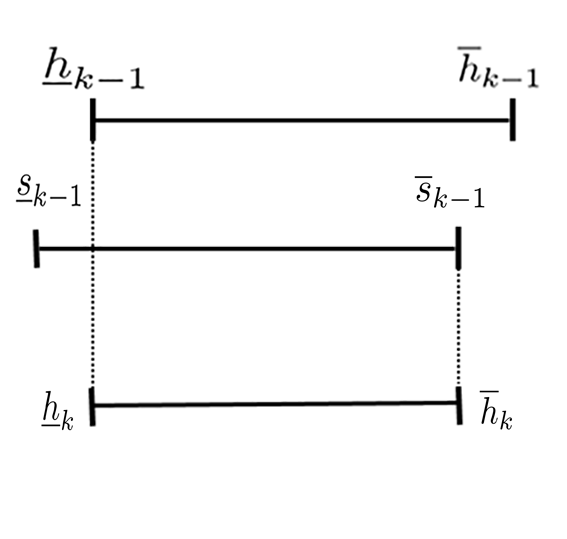
\includegraphics[width=0.5\textwidth ]{ch2-1d-export.png}\\	 % e.g.,[scale=0.75], [width=0.75\textwidth ]
	\caption{$d_{1}=1$时,信息浓缩过程的几何解释}
	\label{fig.1d.export}
\end{figure}

\subsubsection{多维参数情形}\label{subsubsect:2.3.3.2}
当$d_{1}>1$时,$\bm{\theta}$和$\bm{\phi_{k}}$都是向量,和方程\eqref{eq.Ik.d1}类似可以得到
\begin{equation}%
\label{eq.the.phi.d2}
\bm{\phi}_{k-1}^{T}\bm{\theta}\in[y_{k}-u_{k-1}-\overline{z},y_{k}-u_{k-1}-\underline{z}].
\end{equation}
上面的区间形式可以写成下面关于参数向量$\bm{\theta}$的两个不等式
\begin{equation}%
\label{eq.the.phi.d2}
\begin{split}%
\bm{\phi}_{k-1}^{T}\cdot\bm{\theta}&\leq y_{k}-u_{k-1}-\overline{z}\\
(-\bm{\phi}_{k-1}^{T})\cdot\bm{\theta}&\leq -(y_{k}-u_{k-1}-\underline{z})
\end{split}
\end{equation}

从几何上看,方程组\eqref{eq.the.phi.d2}中的任意一个线性不等式的解,都代表着一个定义在域$\mathcal{R}^{d}$上的广义半平面。因此,通常来说,关于同一向量$\bm{\theta}$的多个线性不等式的解在在几何上表示为一个广义多边形或者多面体,仅需要找出这个多面体的顶点(向量描述)就可确定这个多面体。特别的,$d=2$时,多个方程组\eqref{eq.the.phi.d2}的解就是平面上的一个普通多边形,确定了这个多边形的顶点就等价于确定了参数满足的集合$C_{k}$。

记
\begin{equation}%
\label{eq.Vk}
\Gamma_{k}=\{P_{n},n=1,2,\ldots,N_{k}\}
\end{equation}
为定义在区域$C_{k}$上的多面体顶点集合,其中$P_{n}$代表某个顶点,第$k$时刻集合$\Gamma_{k}$包含$N_{k}$个顶点。这里$\Gamma_{k}$记为一个多面体。这里的顶点集情况是对于$d_{1}>2$时有意义。下面先给出多维情形的一般公式。

由方程\eqref{eq.CkIk}可知,从约束条件来看,集合$C_{k}$比$C_{k-1}$多了一组不等式
\begin{equation}%
\label{eq.nq.d2}
\begin{split}%
\bm{\phi_{k-1}}^{T}&\cdot\bm{\theta}\leq v_{k,1}\\
(-\bm{\phi_{k-1}}^{T})&\cdot\bm{\theta}\leq v_{k,2}
\end{split}
\end{equation}
其中
\begin{equation}%
\label{eq.fk}
\begin{split}%
v_{k,1}&=y_{k}-u_{k-1}-\underline{z}\\
v_{k,2}&=-(y_{k}-u_{k-1}-\overline{z})
\end{split}
\end{equation}
本文称\eqref{eq.nq.d2}为线性约束。和$d_{1}=1$情形类似,可以得到信息约束的递推形式为
\begin{equation}%
\begin{split}%
\Gamma_{k-1}'&=G(\Gamma_{k-1},\bm{\phi_{k-1}},v_{k,1})\\
\Gamma_{k}&=G(\Gamma_{k-1}',\bm{\phi_{k-1}},v_{k,2})
\end{split}
\end{equation}
这里$G(\Gamma,\bm{\phi},f)$代表一种变换(算法),它表示在初始的多面体$\Gamma$中加入一个线性约束条件$\bm{\phi}\cdot\bm{\theta}\leq e$。

图\ref{fig.2d.export}展示了$d_{1}=2$时$G$变换的过程。图中,原有的参数区域是由顶点集
\begin{equation}%
\{P_{1},P_{2},P_{3},P_{4},P_{5}\}
\end{equation}
围成的多边形,加入线性约束条件$\bm{\phi}\cdot\bm{\theta}\leq e$之后,变成了顶点集
\begin{equation}%
\{P_{1}',P_{2}',P_{3},P_{4},P_{5}\}
\end{equation}
围成的多边形(深色部分)。

\begin{figure}[htb]
	\centering
	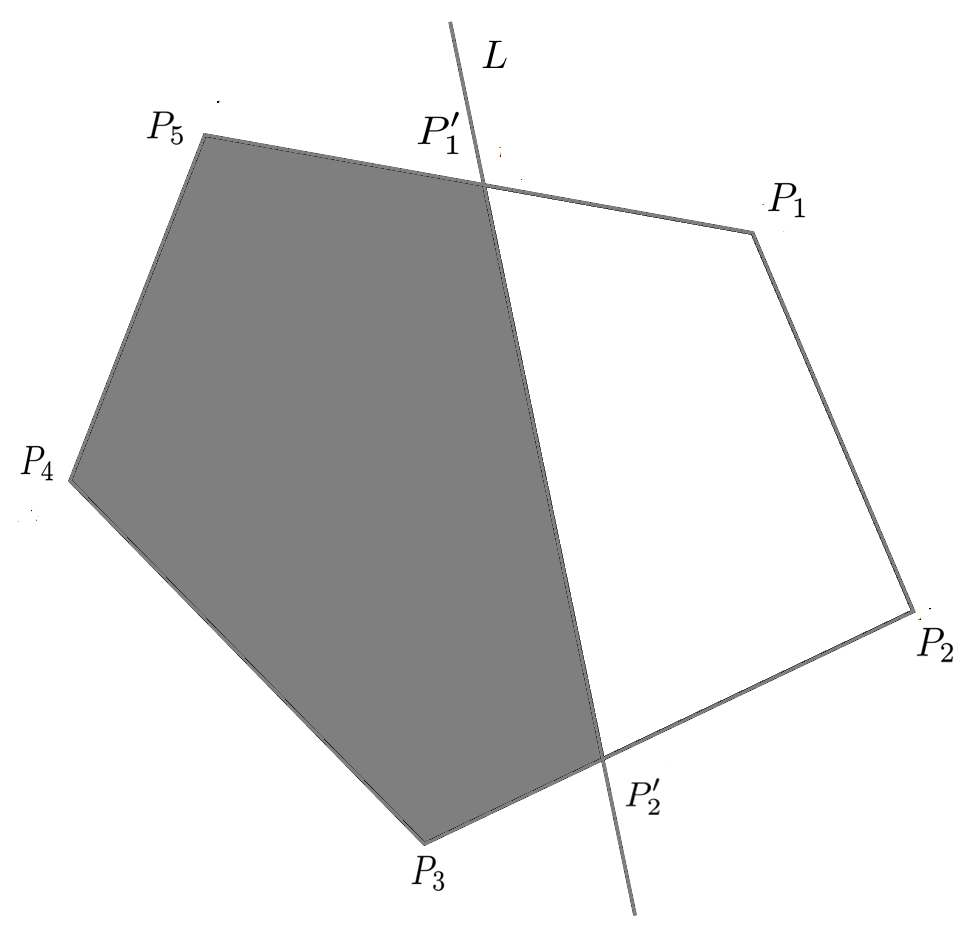
\includegraphics[width=0.5\textwidth ]{ch2-2d-export.png}\\	 % e.g.,[scale=0.75], [width=0.75\textwidth ]
	\caption{$d_{1}=2$时,信息浓缩$G$变换过程的几何解释}
	\label{fig.2d.export}
\end{figure}

可以看出,多边形的面积在原来的基础上缩小了,即参数的可行域减少了,参数不确定性随着也就减少了。不过图\ref{fig.2d.export}只是线性约束和多边形位置的一种情况,因为很可能直线$L$和多边形没有交点,那么经过这个时刻的信息浓缩后,参数集合不变。因此在设计算法实现时需要考虑周全,否则可能导致$C_{\infty}=\varnothing$的出现。

$d_{1}>2$时高维情形的情况类似,只是多边形变成了多面体,直线变成了广义半平面,由于多维情形不容易形象描述,此处就不再一一画出图形说明,留给读者自己想象。

\section{本章总结}
本章的主要内容是半参数系统和信息浓缩估计的基本思想。首先由关于已有的反馈机制能力极限的探索引出存在的不确定性系统的自适应控制问题;然后从实际问题抽象出半参数系统的基本模型,介绍了相关的先验知识举例;接着介绍了一种基于集合的参数估计算法即所谓的信息浓缩估计的主要思想;最后针对典型系统介绍了信息浓缩估计的具体实施框架。